%Compilation sous FreeBSD:
% pkg install tex-formats tex-xetex
% xelatex TP_GIF_SSH_OpenVPN.tex
%Compilation sous MacOS:
% brew install --cask mactex
% TexShop, selectionner le moteur XeLaTeX
%Style de document (format papier, taille police, langue)
\documentclass[a4paper,11pt]{article}
%New command "shellcmd" for CLI command style
\newcommand{\shellcmd}[1]{\texttt{#1}}
%New command "question" for Question formating
\newcommand{\question}[1]{\begin{center}\textbf{#1}\end{center}}
%New command "cadre" for drawing a box
\newcommand{\cadre}[1]{\framebox{\begin{minipage}{0.95\linewidth}\ #1\end{minipage}}}
%Define a variable used for the question numbers
\newcounter{saveenum}
%Suppression des marges
%On ajoute la largeur des marges au text
\addtolength{\textwidth}{\marginparwidth}
\addtolength{\textwidth}{\marginparsep}
\addtolength{\textwidth}{\oddsidemargin}
%Puis on réduis les marges à 0
\marginparwidth=0cm
\oddsidemargin=0cm
\marginparsep=0cm
%On enlève même 1cm à la marge de droite et on ajoute 2cm à la largeur du texte (pour aussi gagner 1cm sur la marge de gauche)
\addtolength{\hoffset}{-1cm}
\addtolength{\textwidth}{2cm}
%Idem pour les hauteurs de marges: Suppression complète de l'entête
\addtolength{\textheight}{\topmargin}
\addtolength{\textheight}{\headheight}
\addtolength{\textheight}{\headsep}
\topmargin=0cm
\headheight=0cm
\headsep=0cm
%On enlève même 1cm à la marge du haut et on ajoute 2cm à la longueur du texte (pour aussi gagner 1cm sur la marge du bas)
\addtolength{\voffset}{-1cm}
\addtolength{\textheight}{2cm}
%Verify the layout (need to use \layout in the document)
%\usepackage[francais]{layout}
%Support du francais
\usepackage{fontspec}
\usepackage{polyglossia}
\setmainlanguage{french}
%polyglossia ajoute des espaces avant les points : ! ? mais on n'en veux pas toujours
\makeatletter
\newcommand{\nospace}[1]{\nofrench@punctuation\texttt{#1}\french@punctuation}
\makeatother
%Permet de formatter les URLs correctements
\usepackage{hyperref}
%Permit to insert image with includegraphics
\usepackage{graphicx}
%Permit to insert EPS graphic file
\usepackage{epstopdf}
%Declare path for all picture files
\graphicspath{ {schemas/} }
%Commande				Niveau
%\part{partie}				-1
%\chapter{chapitre}			0
%\section{section}				1
%\subsection{sous-section}		2
%\subsubsection{sous-sous-section}	3
%\paragraph{paragraphe}		4
%\subparagraph{sous-paragraphe}	5
%Numéro de page en bas (défaut)
\pagestyle{plain}
\author{Olivier Cochard-Labbé}
\title{TP Réseau et Sécurité - IUT St Malo}
\begin{document}
%Pour afficher une page indiquant le type de marge et leur valeurs
%\layout
% generates the title
\maketitle
% insert the table of contents
%Insertion d'un warning: pas possible de lire sur un téléphone
\centerline{
{\Large
{\fontencoding{U}\fontfamily{futs}\selectfont\char 66\relax}
Document non lisible sur smartphone (taille A4 minimum)
}
}
\tableofcontents
\clearpage
% Si latex ne peut couper un mot, alors il le met à la ligne et ne dépasse pas dans la marge
\sloppy
\section{Présentation du TP GIF, SSH et OpenVPN}
Ce TP se découpe en plusieurs exercices du plus simple au plus complexe, tous présentant différentes méthodes pour mettre en place un VPN (interconnexion de réseau privé au-dessus d'un réseau public) :
\begin{enumerate}
\item  Mise en place de la maquette : permet de découvrir le paramétrage du système d'exploitation FreeBSD;
\item Tunnel GIF pour de l'encapsulation IP dans IP sans chiffrage;
\item Client SSH en redirection de flux TCP avec authentification par clés SSH ;
\item Configuration d'un serveur SSH et génération de clé SSH (exercice par paire de binôme) ;
\item Configuration d'un client OpenVPN authentifié par certificats;
\item Configuration d'un serveur OpenVPN et la création/répudiation de certificat (exercice par paire de binôme).
\end{enumerate}
\subsection{Grille de notation}
La différence entre deux techniciens se fait uniquement à la qualité du travail écrit rendu. La notation de votre rapport prendra donc en compte:
\begin{enumerate}
\item La documentation de l'ensemble de vos actions. Ce qui inclut la description des commandes passées pour la préparation de vos environnements, le nettoyage éventuellement nécessaire entre les différents exercices, les exercices eux-mêmes et vos résolutions de problèmes rencontrés;
\item La réponse aux questions numérotées;
\item Avec quelques points supplémentaires pour toutes réponses aux questions IPv6.
\end{enumerate}
Vous noterez qu'il est donc possible de réussir l'intégralité des exercices proposés, mais au final c'est uniquemement le contenu de votre rapport qui sera noté.


Concernant l'insertion de captures d'écrans qui sont fortement conseillées:
\begin{itemize}
\item Elles seront au format bitmap (graphique) si la source de donnée est graphique (capture d'écran de l'environnement graphique des fenêtres Wireshark ou du navigateur);
\item Elles seront au format texte (simple copier/coller) si la source de donnée est le texte du terminal (vos commandes et leurs résultats, fichiers de configuration commentés, extraits de man page ou de fichiers de logs).
\end{itemize}

\clearpage
\subsection{Environnement simulé}
L'environnement du TP simule le réseau du siège d'une entreprise reliée par VPN à ses succursales à travers un réseau public (ici Internet):
\begin{center}
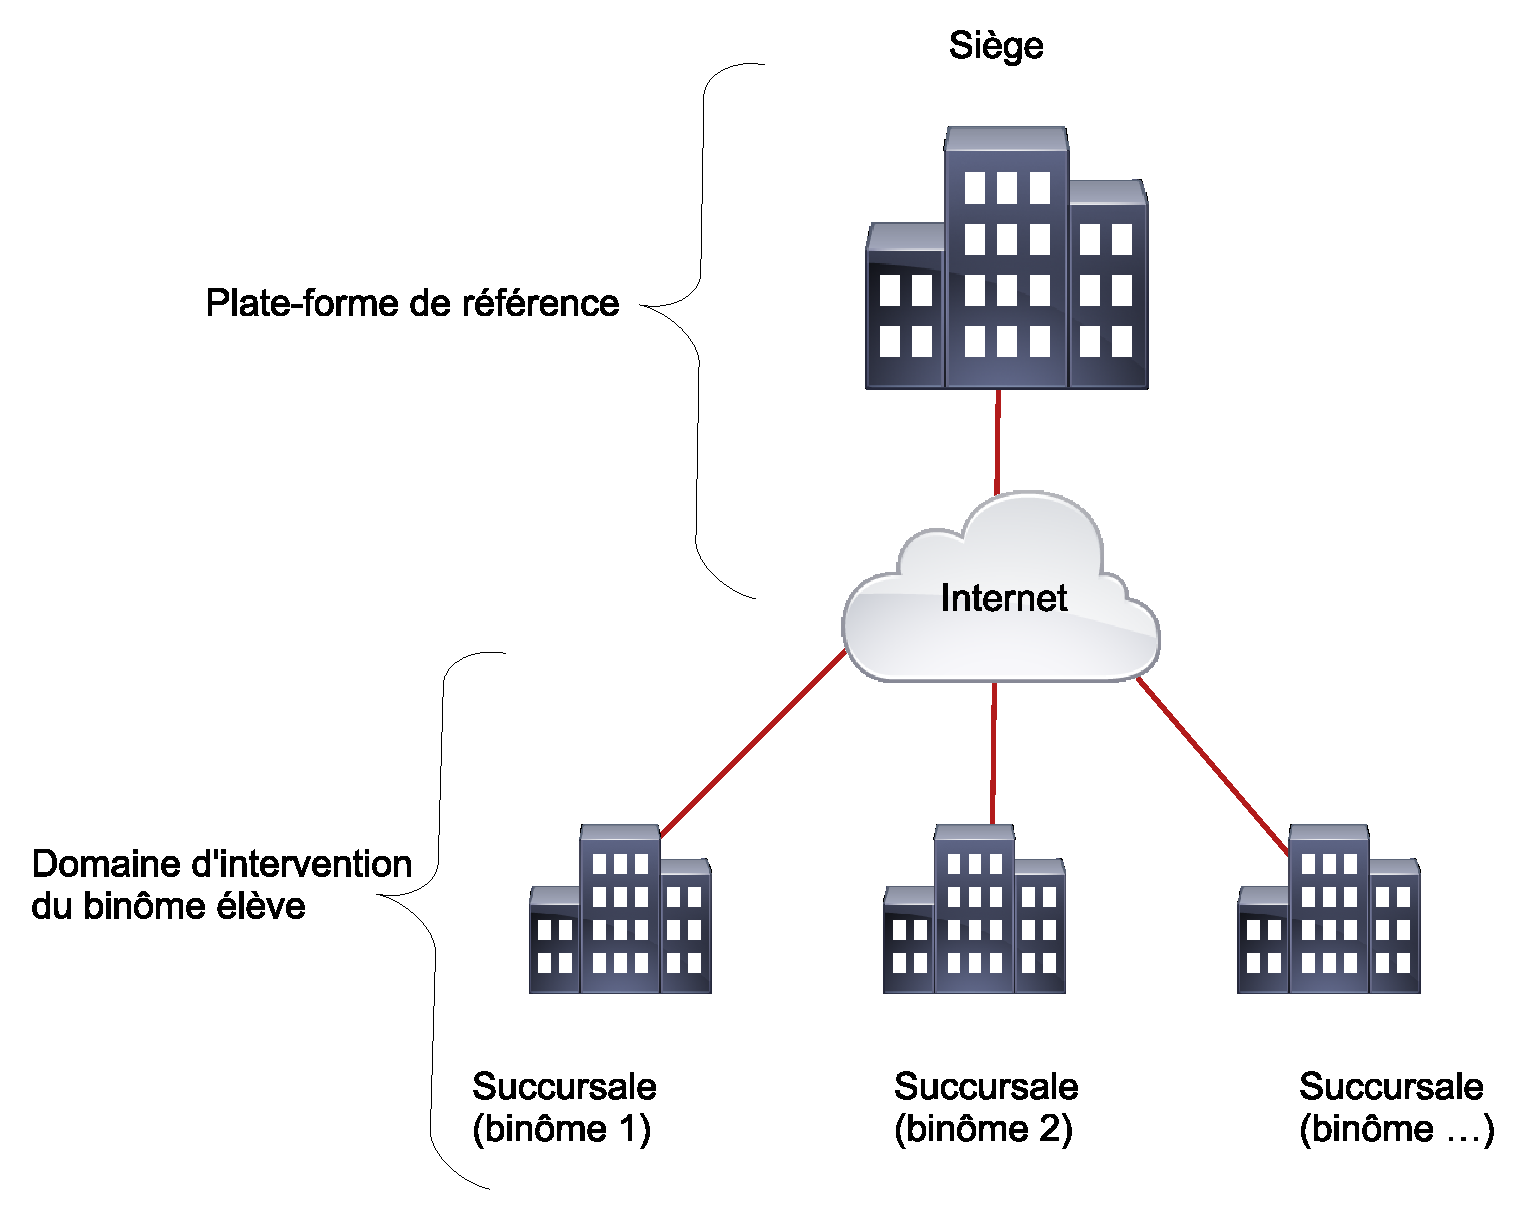
\includegraphics[width=0.6\linewidth]{environnement-simule}
\end{center}
%\clearpage
\subsection{FreeBSD}
Ce TP utilise un système d'exploitation libre de la famille des Unix\footnote{GNU/Linux n'est pas un Unix.}. L'avantage d'utiliser FreeBSD dans notre cas est sa simplicité de configuration (très peu de fichiers de configuration à modifier) ainsi que sa documentation très complète (pages man et guide utilisateur). De plus, la robustesse de sa pile IP et sa licence BSD en fait un système très couramment utilisé sur les équipements réseau et appliances (routeurs et commutateurs Juniper, Firewall Netasq, NAS NetApp et Isilon, Netflix OpenConnect, console Sony PS4, etc.).

Particularité de FreeBSD pour les habitués à GNU/Linux : Le nom des périphériques (interfaces réseau, disques, etc…) n'est pas identifié par des noms génériques (eth0 pour la première carte réseau) mais par des noms liés aux drivers utilisés (bge0 pour la première carte Ethernet utilisant un pilote Broadcom, fxp0 pour une carte réseau Intel EtherExpress PRO/100, em0 pour des Intel Pro/1000, etc…).

Pour afficher la liste des interfaces réseau détectées, utilisez la commande \shellcmd{ifconfig} sans argument.

Voici la description de la sortie da la commande \shellcmd{ifconfig nom-interface}:
\footnotesize
\begin{verbatim}
[etudiant@routeur]~>ifconfig em0
em0: flags=8843<UP,BROADCAST,RUNNING,SIMPLEX,MULTICAST> metric 0 mtu 1500      => État logique
        options=9b<RXCSUM,TXCSUM,VLAN_MTU,VLAN_HWTAGGING,VLAN_HWCSUM>          => Fonctionnalités activées
        ether 08:00:27:e3:9b:3f                                                => Adresse MAC
        inet6 fe80::a00:27ff:fee3:9b3f%em0 prefixlen 64 scopeid 0x1            => IPv6 link-local
        inet 2.2.2.15 netmask 0xffffff00 broadcast 2.2.2.255                 => Adresse IPv4
        inet6 fc00:10::254 prefixlen 64                                        => Autre IPv6
        nd6 options=3<PERFORMNUD,AUTO_LINKLOCAL>                               => Options ND IPv6
        media: Ethernet autoselect (1000baseT <full-duplex>                    => auto-négociation physique
        status: active                                 => État physique de l'interface (présence d'un câble)
                                                          (Valide uniquement si l'interface est à l'état UP)
\end{verbatim}
\normalsize
Voici quelques autres commandes qui vont vous être utiles pour l'ensemble de ce TP:
\begin{itemize}
\item Afficher la liste des routes : \shellcmd{netstat -rn}
\item Passer super-utilisateur (root) : \shellcmd{su -}
\item Afficher le manuel d'une commande : \shellcmd{man commande}
\item Afficher/modifier la liste des paramètres noyaux : \shellcmd{sysctl}
\item Afficher, en temps réel, un fichier : \shellcmd{tail -f /var/log/messages}
\item Afficher les dernières lignes d'un fichier : \shellcmd{tail /var/log/messages}
\item Désarchiver un fichier .tgz : \shellcmd{tar zxvf nom-du-fichier.tgz}
\end{itemize}
Pour plus d'information, se référer à la version anglaise (une traduction ne sera jamais à jour) du guide utilisateur sur \textbf{www.freebsd.org/doc/en/books/handbook/}.

Sur la clé USB amorçable qui vous a été remise, vous y trouverez une installation standard de FreeBSD incluant les outils de base comme OpenSSH, \shellcmd{tcpdump}, \shellcmd{vi}, \shellcmd{ee} ainsi que les logiciels additionnels suivants :
\begin{itemize}
\item OpenVPN;
\item mohawk: serveur web;
\item vim et nano: Éditeurs de texte supplémentaires;
\item w3m: navigateur web en mode texte (console).
\end{itemize}
Voici les paramètres de connexion pour se connecter à la console :
\begin{itemize}
\item login du compte utilisateur : \shellcmd{etudiant}
\item mot de passe du compte utilisateur : \shellcmd{iut}
\item mot de passe du compte root : \shellcmd{stmalo}
\end{itemize}
\emph{N'utiliser le compte «~root~» que quand c'est obligatoire, c'est-à-dire pour la modification de fichier de configuration système ou le lancement de daemon.}
\subsubsection{Éditeurs de texte}
FreeBSD propose par défaut deux éditeurs de texte :
\begin{itemize}
\item \shellcmd{vi} : Éditeur Unix classique mais complexe pour un débutant (si vous ne le connaissez pas, ne perdez pas de temps à le découvrir pendant ce TP) ;
\item \shellcmd{ee} (easy editor) : Éditeur plus simple qui convient mieux aux débutants.
\end{itemize}
Pour éditer un fichier texte avec ee, exécuter la commande \shellcmd{ee mon-fichier.txt} pour se retrouver sur un écran séparé en 2 sections haut/bas :
\footnotesize
\begin{verbatim}
^[ (escape) menu  ^y search prompt  ^k delete line   ^p prev li   ^g prev page
^o ascii code     ^x search         ^l undelete line ^n next li   ^v next page
^u end of file    ^a begin of line  ^w delete word   ^b back 1 char
^t top of text    ^e end of line    ^r restore word  ^f forward 1 char
^c command        ^d delete char    ^j undelete char ^z next word
=====line 1 col 0 lines from top 1 ============================================






new file "mon-fichier.txt"
\end{verbatim}
\normalsize
La première section du haut rappel la liste des commandes possibles. Par exemple elle indique que pour afficher le menu il faut appuyer sur la touche escape. Le caractère \textasciicircum \ indique de garder enfoncé la touche contrôle (Ctrl) pendant que vous appuierez sur la touche correspondante. Par exemple, pour lancer la recherche d'un mot, c'est la combinaison Ctrl + y.
\subsubsection{Organisation de la configuration}
L'organisation détaillée des dossiers est expliquée dans \shellcmd{man hier}:
\begin{itemize}
\item L'ensemble de la configuration du système de base se trouve dans le dossier /etc;
\item La configuration des applications additionnelles (OpenVPN, easyrsa, vim, nano dans notre cas) se trouve dans le dossier /usr/local/etc.
\end{itemize}
Les paramètres globaux (nom de machine, adresses IP, routes par défaut et statiques, démarrage des services, etc.) seront a déclarer dans le fichier /etc/rc.conf.
Pour découvrir les différentes options de ce fichier, inspirez-vous du fichier /etc/defaults/rc.conf qui contiens l'ensemble des paramètres par défaut ainsi que des exemples (mais ne jamais modifier ce fichier !). La configuration des paramètres spécifiques à certains daemons se fait dans leurs dossiers relatifs (/etc/ssh/sshd\_config pour le serveur openssh par exemple).

\cadre{\question{Question}
\begin{enumerate}
\item Quel est l'intérêt d'avoir une séparation nette entre les composants du système d'exploitation et les applications tierces ?
\setcounter{saveenum}{\value{enumi}}
\end{enumerate}
}
\subsubsection{Présentation de la gestion de la configuration et des services par l'activation de sshd}
Il est possible d’afficher et modifier le contenu du fichier /etc/rc.conf sans passer par un éditeur texte en utilisant la commande \shellcmd{sysrc} :
\begin{itemize}
\item Ajoute ou modifie la variable dans /etc/rc.conf: \shellcmd{sysrc variable=valeur}
\item Active un service: \shellcmd{service NOM-DU-SERVICE enable}
\item Affiche la liste des variables modifiées: \shellcmd{sysrc -a}
\end{itemize}
Commencer par activer le daemon SSH :
\begin{enumerate}
\item Ajouter la ligne \shellcmd{sshd\_enable="YES"} dans le fichier /etc/rc.conf ou en utilisant la commande \shellcmd{service sshd enable};
\item Lancer le démarrage du service par la commande \shellcmd{service sshd start}.
\end{enumerate}
Lors du lancement de celui-ci, il va générer différentes clés SSH pour lui-même et afficher l'emprunte de ces clés: Notez-les car elles vous seront demandées ultérieurement.

Les scripts de démarrage des services systèmes se trouvent dans /etc/rc.d et ceux des applications tierces (OpenVPN, mohawk) dans /usr/local/etc/rc.d. Il est possible d'afficher la liste complète des scripts RC disponibles par la commande \shellcmd{service~-l} et d'afficher la liste des services activés par la commande \shellcmd{service~-e}.

Remarques concernant quelques services systèmes particuliers :
\begin{itemize}
\item Applique une création/modification d'interface réseau: \shellcmd{service netif restart}
\item Applique une modification de routes: \shellcmd{service routing restart}
\end{itemize}

\cadre{\question{Questions}
\begin{enumerate}
\setcounter{enumi}{\value{saveenum}}
\item Quelle est la commande pour vérifier l'état d'un service (lancé/arrêté) ?
\item Vérifiez l'état du démon SSH.
\setcounter{saveenum}{\value{enumi}}
\end{enumerate}
}
\subsection{Interfaces virtuelles TUN et TAP}
Une interface virtuelle est une interface logique qui dans notre cas sert à représenter les tunnels VPN.

\cadre{\question{Questions}
\begin{enumerate}
\setcounter{enumi}{\value{saveenum}}
\item Quel autre type d'interface virtuelle existe-t-il par défaut sur toute machine Linux/Unix ?
\item À l'aide des commandes \shellcmd{man tun} et \shellcmd{man tap}, détaillez la différence entre ces interfaces;
\item Les exercices sur OpenVPN nécessiteront uniquement des interfaces virtuelles routées: Quel type d'interface allez-vous utiliser pour ces exercices?
\setcounter{saveenum}{\value{enumi}}
\end{enumerate}
}
%\clearpage
\section{Exercice : Mise en place de la maquette}
\subsection{Schéma complet}
Voici le schéma logique de la maquette :
\begin{center}
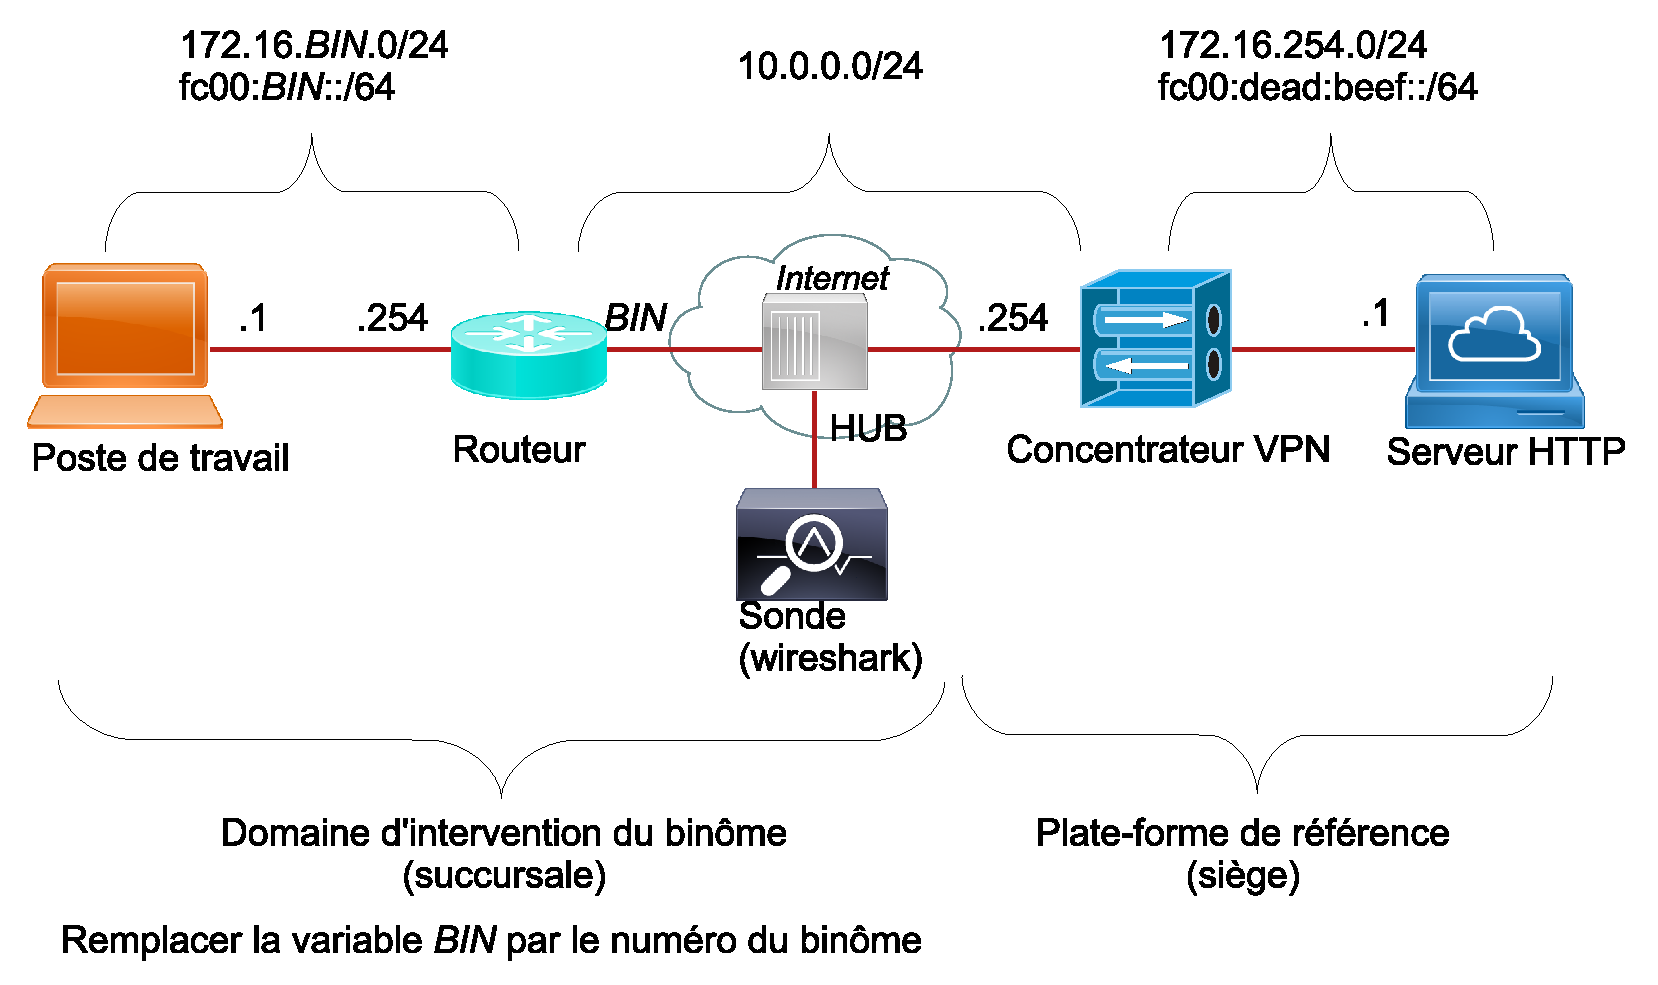
\includegraphics[width=0.9\linewidth]{schema-complet}
\end{center}

Note : Définissez un numéro de binôme (entre 1 et 20) unique entre vous. Aux adresses hôtes IPv4 notées .254, vous utiliserez l'équivalent visuel en IPv6 (par exemple l'adresse IPv6 interne du routeur binôme 20 est \shellcmd{fc00:20::254/64} et l'IPv4 : \shellcmd{172.16.20.254/24}).

\subsection{Votre environnement}
Pour la réalisation de ce TP vous utiliserez 2 PCs :
\begin{itemize}
\item Un premier PC avec 2 cartes réseau que vous démarrerez sur la clé USB fournie : Il jouera le rôle de PC «~routeur VPN~»;
\item Un second PC avec 2 cartes réseau qui jouera le rôle de PC «~poste client et sonde~». Vous démarrerez ce PC sous Linux en prévoyant d'être capable d'y lancer un navigateur (pour les exercices «~client SSH~» et «~client VPN~») ainsi qu'un serveur HTTP (pour les exercices «~serveur SSH~» et «~serveur VPN~»).
\end{itemize}
\begin{center}
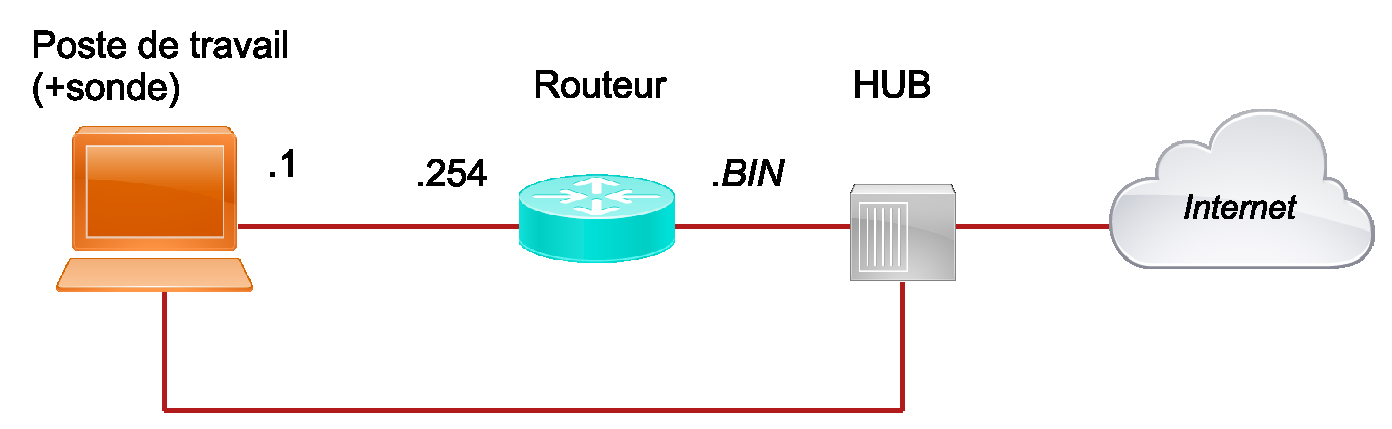
\includegraphics[width=0.8\linewidth]{environnement}
\end{center}
\subsection{Paramétrage initial du PC «~poste de travail et sonde~»}
Nous allons commencer par le plus simple qui est le paramétrage IP du PC «~poste de travail~» :
\begin{enumerate}
\item Identifier les interfaces Ethernet correspondantes à votre maquette ;
\item Configurer les adresses IP sur l'interface Ethernet reliée au «~ PC routeur~» ;
\item Déclarer la (les?) route(s) par défaut ;
\item Désactiver l'émission de requête IPv6 RA et AUTOCONF sur l'interface Ethernet utilisée comme sonde par les commandes \shellcmd{sysctl net.ipv6.conf.eth??.accept\_ra=0} et \shellcmd{sysctl net.ipv6.conf.eth??.autoconf=0};
\item Lancer la capture de trafic sur l'interface Ethernet utilisée comme sonde ;
\end{enumerate}
\cadre{\question{Questions}
\begin{enumerate}
\setcounter{enumi}{\value{saveenum}}
\item Quel est le mode d'attribution d'IPv6 le plus logique à mettre en œuvre pour un poste de travail ?
\setcounter{saveenum}{\value{enumi}}
\end{enumerate}
}
\subsection{Paramétrage du PC «~routeur~»}

\emph{Lisez l'ensemble de ce chapitre avant de commencer à manipuler.}

Pour paramétrer le PC «~routeur~» les tâches à effectuer sont celles-ci :
\begin{enumerate}
\item Identifier les interfaces Ethernet correspondantes à votre maquette ;
\item Affecter les bonnes adresses IP sur les bonnes interfaces ;
\item Activer le routage IPv4 et IPv6 (ainsi que le daemon rtadvd pour IPv6) ;
\end{enumerate}
L'identification des interfaces Ethernet peut-être réalisée en suivant cette méthode :
\begin{enumerate}
\item Activer les interfaces Ethernet : \shellcmd{ifconfig INTERFACE up};
\item Débranchez physiquement tous les câbles Ethernet sauf un ;
\item À l'aide de l'état des interfaces, champ status du résultat de la commande \shellcmd{ifconfig}, identifiez l'unique interface physique qui possède le status «~active~».
\end{enumerate}
Le paramétrage IP se résume simplement à déclarer les bonnes valeurs des bonnes variables dans le fichier /etc/rc.conf et à redémarrer les services impactés pour la prise en compte des changements.
Voici la liste les variables utiles dans notre cas (inspirez-vous du fichier /etc/defaults/rc.conf pour connaître leur description et les valeurs à utiliser) :
\begin{verbatim}
ifconfig_??="inet ??/??"
gateway_enable="??"
ipv6_activate_all_interfaces="YES"
ipv6_gateway_enable="??"
ifconfig_??_ipv6="inet6 ?? prefixlen ??"
rtadvd_enable="??"
rtadvd_interfaces="??"
\end{verbatim}
Une fois le fichier modifié, relancez les services impactés :
\begin{verbatim}
service netif restart
service routing restart
service rtadvd restart
\end{verbatim}
\cadre{\question{Questions}
\begin{enumerate}
\setcounter{enumi}{\value{saveenum}}
\item Quel(s) test(s) effectuez-vous pour valider le fonctionnement du routage ? (la réponse n'est pas simple)
\item Il était aussi possible de paramétrer votre système avec les commandes \shellcmd{ifconfig} ou  \shellcmd{route}. Quelle est la différence entre le fait d'utiliser ces commandes et modifier le fichier de configuration puis de relancer les services  ?
\setcounter{saveenum}{\value{enumi}}
\end{enumerate}
}
\\
\\\emph{\\Appelez-les tuteurs pour qu'ils valident l'état de votre maquette et qu'ils vous transfèrent vos clés SSH et certificats OpenVPN dans le dossier /home/etudiant/.}
%\clearpage
\section{Exercice : Tunnel GIF - Encapsulation IP dans IP}
Cette méthode utilise le protocole GIF (RFC2893 : encapsulation de datagramme IP dans IP sans chiffrement) pour créer un VPN :
\begin{center}
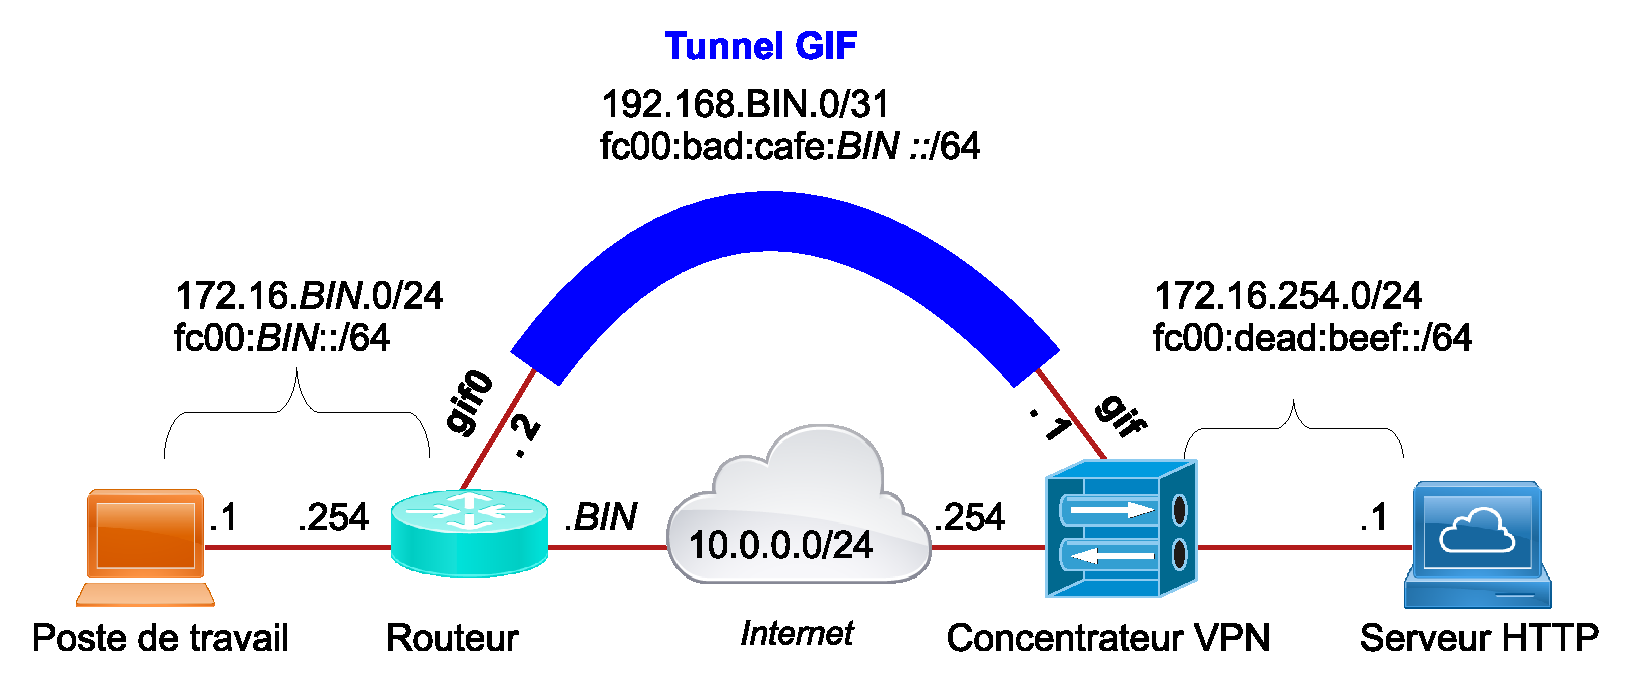
\includegraphics[width=\linewidth]{Tunnel-GIF}
\end{center}

Référez-vous à la man page GRE plutôt que celle de GIF pour les explications détaillées du concept d'encapsulation et de son paramétrage par la commande \shellcmd{man gre}. La déclaration d'une interface GIF se réalise avec ces deux lignes de configurations dans le fichier /etc/rc.conf:
\footnotesize
\begin{verbatim}
cloned_interfaces="gif0"
ifconfig_gif0="inet INNER-LOCAL-IP/MASK INNER-REMOTE-IP tunnel OUTER-LOCAL-IP OUTER-REMOTE-IP up"
ifconfig_gif0_ipv6="???"
\end{verbatim}
\normalsize
Ne pas oublier la déclaration des routes statiques pour atteindre le réseau du siège.

\cadre{\question{Questions}
\begin{enumerate}
\setcounter{enumi}{\value{saveenum}}
\item Quelles adresses IP sont à attribuer à cette nouvelle interface virtuelle?
\item Quelles routes statiques sont à ajouter pour atteindre le serveur Web du siège en utilisant ce tunnel?
\item Montrez sur une capture de trame l'encapsulation des paquets et les différentes adresses IP contenues dans un paquet GIF.
\setcounter{saveenum}{\value{enumi}}
\end{enumerate}
}

Une fois le paramétrage IP terminé, à partir du navigateur du PC «~poste de travail~», il est possible de joindre les URL suivantes:
\begin{itemize}
\item \url{http://172.16.254.1}
\item \url{http://[fc00:dead:beef::1]}
\end{itemize}
\emph{Appelez-les tuteurs pour qu'ils valident l'état de votre maquette.}
%\clearpage
\section{Exercice : Client SSH - Protection de flux TCP}
Cet exercice présente une première utilisation de SSH par la protection de flux TCP.
L'administrateur réseau du siège a réalisé deux actions :
\begin{enumerate}
\item Il a créé un compte utilisateur (login : succursale\_BIN, mot de passe : BIN) sur le concentrateur VPN du siège;
\item Il vous a transmis une archive (succursale\_BIN\_cles.tgz) contenant les clés SSH (privée et publique) et certificat OpenVPN de l'utilisateur ainsi que l'emprunte SSH de la clé du concentrateur VPN (dans le dossier /home/etudiant).
\end{enumerate}
\emph{Rappel : Ne travaillez sous le compte root que quand c'est ABSOLUMENT utile.}
\\
Désarchiver votre archive contenant les clés SSH.

\cadre{\question{Questions}
\begin{enumerate}
\setcounter{enumi}{\value{saveenum}}
\item Quelle est la clé, a préciser dans la commande ssh, qui est utilisée pour chiffrer votre session à destination du siège ?
\item Comme il faut 2 clés pour chiffrer, quelle est la deuxième clé utilisée automatiquement par SSH et comment la récupère-t-il?
\item Quelle est sont les clés déja installées sur le serveur SSH du siège qui vont être utilisés pour déchiffrer vos messages ?
\item Quelle est l'autorité de certification ?
\item Qu'est-ce qu'une attaque de type «~man in the middle~» ? Comment s'en protéger ? et comment SSH protège de ce type d'attaque ?
\setcounter{saveenum}{\value{enumi}}
\end{enumerate}
}

Voici le principe de la redirection d'un port TCP dans une session SSH :
\begin{center}
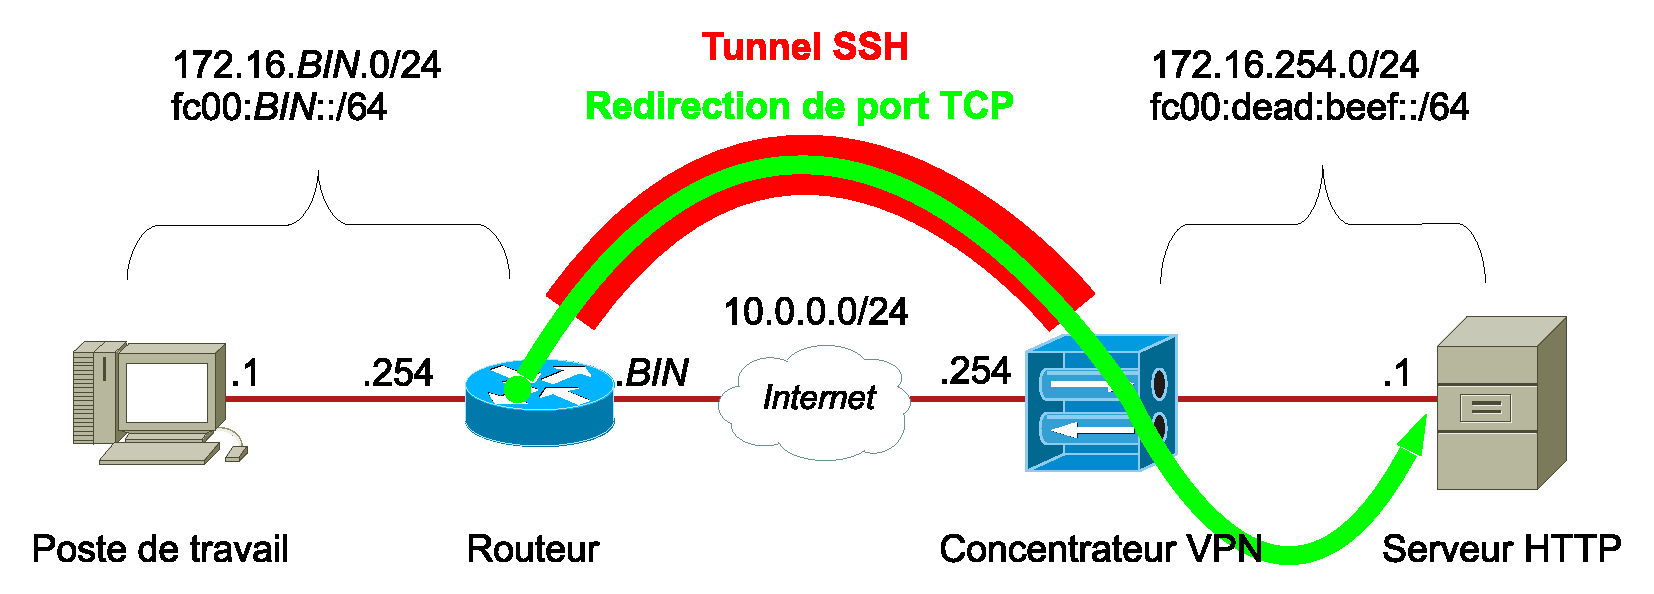
\includegraphics[width=\linewidth]{SSH-redirection}
\end{center}

Le PC «~routeur~» va lancer un tunnel SSH à destination du Concentrateur SSH/VPN et permettre de rediriger le trafic TCP à destination de son propre port 8080, vers le port 80 du serveur HTTP à travers ce tunnel SSH.
Pour activer cette redirection de port, vous allez à partir du PC «~routeur SSH/VPN~» :
\begin{enumerate}
\item Vérifiez que vous travaillez bien sous le compte simple utilisateur et non pas root ;
\item Protéger votre clé privé pour que personne d'autre que votre utilisateur ne puisse y accéder par la commande \shellcmd{chmod 600 id\_rsa}. Le client SSH vérifiera les droits d'accès et refusera d'utiliser une clé dont les permissions d'accès ne sont pas assez restrictives ;
\item Lancer la commande suivante (sur une seule ligne) : \shellcmd{\nospace{ssh -N -L8080:172.16.254.1:80 -g~-i~/chemin/votre.clé.ssh~succursale\_BIN@2.2.2.254}}
\item Puis vérifier le fonctionnement en lançant un navigateur à partir de votre PC «~poste de travail~» à destination de votre routeur SSH/VPN sur son port 8080~:
\url{http://172.16.BIN.254:8080} et/ou \url{http://[fc00:BIN::254]:8080}
\end{enumerate}
\cadre{\question{Questions}
\begin{enumerate}
\setcounter{enumi}{\value{saveenum}}
\item À l'aide de la commande \shellcmd{man ssh}, décrivez le rôle de chaque paramètre;
\item Sur quelle machine le port 8080 est en écoute ?
\item Sur quelle machine le port 80 est en écoute ?
\item La clé SSH que vous avez utilisée est-elle protégée par un mot de passe ? Sinon, pensez-vous que ce soit un problème de sécurité et pourquoi ?
\item Quel est l'unique intérêt d'utiliser une clé SSH non protégée par mot de passe ?
\item Est-ce que l'activation du routage sur le PC «~routeur SSH/VPN~» est obligatoire dans cet exemple précis ?
\setcounter{saveenum}{\value{enumi}}
\end{enumerate}
}
\\\emph{\\Appelez-les tuteurs pour qu'ils valident l'état de votre maquette.}
%\clearpage
\section{Exercice : Serveur SSH – Protection de flux TCP}
Votre rôle est désormais de mettre en place un serveur OpenSSH pour permettre l'accès sécurisé à vos ressources. Pour cela vous réaliserez les actions suivantes:
\begin{enumerate}
\item Activer un serveur HTTP sur votre «~poste de travail~» (qui jouera le rôle de serveur HTTP pour cet exercice);
\item Créer un compte utilisateur ainsi que les clés SSH correspondantes sur votre routeur VPN;
\item Transmettre à votre binôme voisin par la commande \shellcmd{scp} les clés SSH.
\end{enumerate}
\subsection{Création d'un compte utilisateur et de ses clés SSH}
Passer super-utilisateur «~root~» pour pouvoir créer un compte utilisateur par la commande \shellcmd{adduser} puis générer le couple de clé SSH par la commande \shellcmd{ssh-keygen -f utilisateur.cle.ssh}. Notez ensuite l’empreinte de la clé avec la commande \shellcmd{ssh-keygen -l}.
Ajoutez la clé publique de l'utilisateur au fichier /home/UTILISATEUR/.ssh/authorized\_keys (ce fichier est le porte-clés public des utilisateurs autorisés à se connecter) par les commandes :
\begin{enumerate}
\item \shellcmd{mkdir /home/UTILISATEUR/.ssh}
\item \shellcmd{cat clé-publique >> /home/UTILISATEUR/.ssh/authorized\_keys}.
\end{enumerate}
Attention : Les droits d'accès au fichier authorized\_keys doivent être strictement limités en écriture à l'utilisateur pour que le daemon SSHd accepte d'utiliser les clés publiques qui y sont  stockées. Pour appliquer ces restrictions, utiliser la commande \shellcmd{chmod 644 /home/UTILISATEUR/.ssh/authorized\_keys}

\cadre{\question{Question}
\begin{enumerate}
\setcounter{enumi}{\value{saveenum}}
\item Quel est le but de cette restriction sur ce fichier authorized\_keys  ?
\setcounter{saveenum}{\value{enumi}}
\end{enumerate}
}

Transmettez les deux clés à votre binôme voisin par scp (attention à la syntaxe: la commande se termine par deux points!) par la commande \shellcmd{\nospace{scp~NOM-DU-FICHIER~etudiant@IP:}}

Puis vérifiez que votre voisin a bien reçu ses deux clés.

\subsection{Protection de flux TCP (redirection de port dans une session SSH)}
Modifier la configuration de votre serveur SSH (/etc/ssh/sshd\_config) pour :
\begin{enumerate}
\item Désactiver la résolution DNS pour éviter d'attendre le timeout de cette résolution lors de la connexion (UseDNS no);
\item Augmenter le niveau de détail des journaux (LogLevel DEBUG) pour diagnostiquer d'éventuel problème (/var/log/debug.log).
\end{enumerate}
N'oubliez pas de redémarrer le service sshd suite à la modification de la configuration.
Puis vérifier que le binôme voisin accède bien à vos ressources en utilisant la redirection de port : Si un mot de passe autre que celui de la clé privée SSH est demandé, cela veut dire que l'authentification par clé SSH ne fonctionne pas !
\\\\\emph{Appelez-les tuteurs pour qu'ils valident l'état de votre maquette.}
%\clearpage
\section{Exercice : Client OpenVPN – Protection de flux IP}
Dans cet exercice votre routeur montera un tunnel OpenVPN vers le concentrateur VPN:
\begin{center}
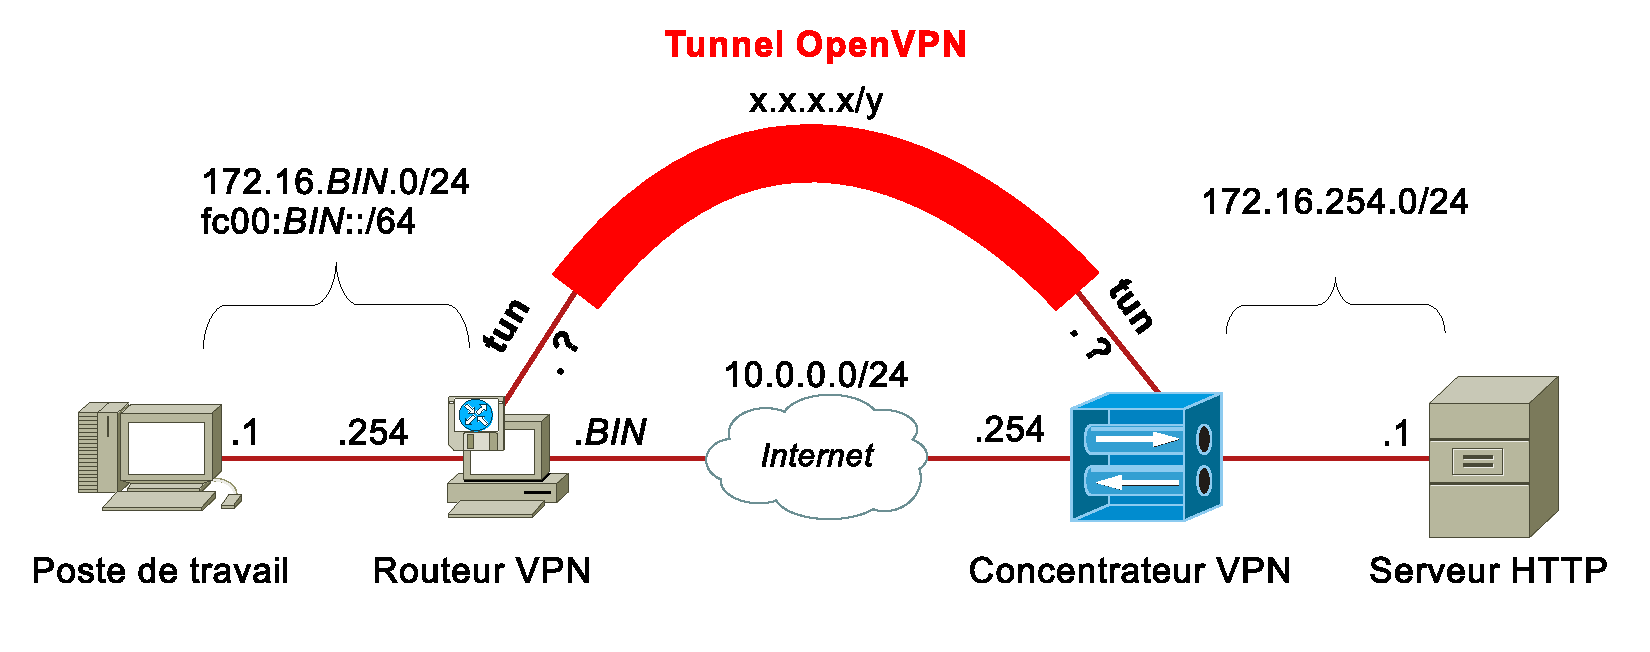
\includegraphics[width=\linewidth]{Tunnel-OpenVPN}
\end{center}
\emph{Détruire les interfaces GIF si elles sont actives avant de réaliser les exercices OpenVPN.}

Pour le paramétrage du client VPN, vous trouverez les certificats OpenVPN dans l'archive transmise par le siège en même temps que les clés SSH.\\
\cadre{\question{Questions}
\begin{enumerate}
\setcounter{enumi}{\value{saveenum}}
\item Détaillez les fichiers présents dans le dossier certifs-openvpn et leurs rôles;
\item Comparez les fichiers relatifs à la cryptographie utilisée par SSH et ceux utilisés par OpenVPN. Quelles sont les équivalences ? Les différences ?
\item Quelle est l'autorité de certification ?
\item Sur quoi repose la «~confiance~» qu'un client peut avoir dans le serveur (pour éviter les attaques «~man in the middle~») dans les deux cas ?
\setcounter{saveenum}{\value{enumi}}
\end{enumerate}
}

Paramétrez le PC «~routeur~» comme client OpenVPN:
\begin{enumerate}
\item Créer le dossier /usr/local/etc/openvpn/;
\item Copiez l'ensemble des certificats OpenVPN qui vous ont été remis dans le dossier /usr/local/etc/openvpn;
\item Inspirez-vous du fichier de configuration d'exemple de client OpenVPN /usr/local/share/examples/openvpn/sample-config-files/client.conf pour créer le fichier de configuration /usr/local/etc/openvpn/succursale.BIN.conf
\end{enumerate}

Les paramètres nécessaires à la configuration de votre client openvpn sont les suivants :
\begin{itemize}
\item Type de service OpenVPN : client
\item Type d'interface virtuelle à utiliser : tun
\item Adresse IP du serveur OpenVPN (remote) : cf le schéma
\item Nom du fichier correspondant au certificat du CA
\item Nom du fichier correspondant à votre certificat «~client~»
\item Nom du fichier correspondant à votre clé «~client~»
\item Le niveau de détail des logs : 4
\end{itemize}
Une fois le fichier de configuration terminé, lancez le client OpenVPN par la commande
\shellcmd{openvpn~/usr/local/etc/openvpn/succursale.BIN.conf}

Vérifiez qu'une nouvelle interface virtuelle a été crée suite au lancement d'OpenVPN.

\cadre{\question{Questions}
\begin{enumerate}
\setcounter{enumi}{\value{saveenum}}
\item Quel est le paramétrage IP de cette nouvelle interface ?
\item En quoi cela a-t-il modifié la table de routage de votre routeur ?
\item Détaillez l'ensemble du journal de connexion indiqué par votre client OpenVPN.
\setcounter{saveenum}{\value{enumi}}
\end{enumerate}
}

Vérifiez ensuite que vous avez accès au serveur Web du siège et mettez en évidence le chiffrage du flux HTTP par votre sonde.
\\\emph{Appelez-les tuteurs pour qu'ils valident l'état de votre maquette.}

%\clearpage
\section{Exercice : Serveur OpenVPN – Protection de flux IP}
\subsection{Les 2 principaux usages d'un tunnel VPN}
Le premier usage d'un tunnel VPN est de connecter un poste nomade aux ressources internes de l'entreprise. Il s'agit du paramétrage le plus simple d'OpenVPN et c'est celui indiqué dans les fichiers d'exemples:
\begin{center}
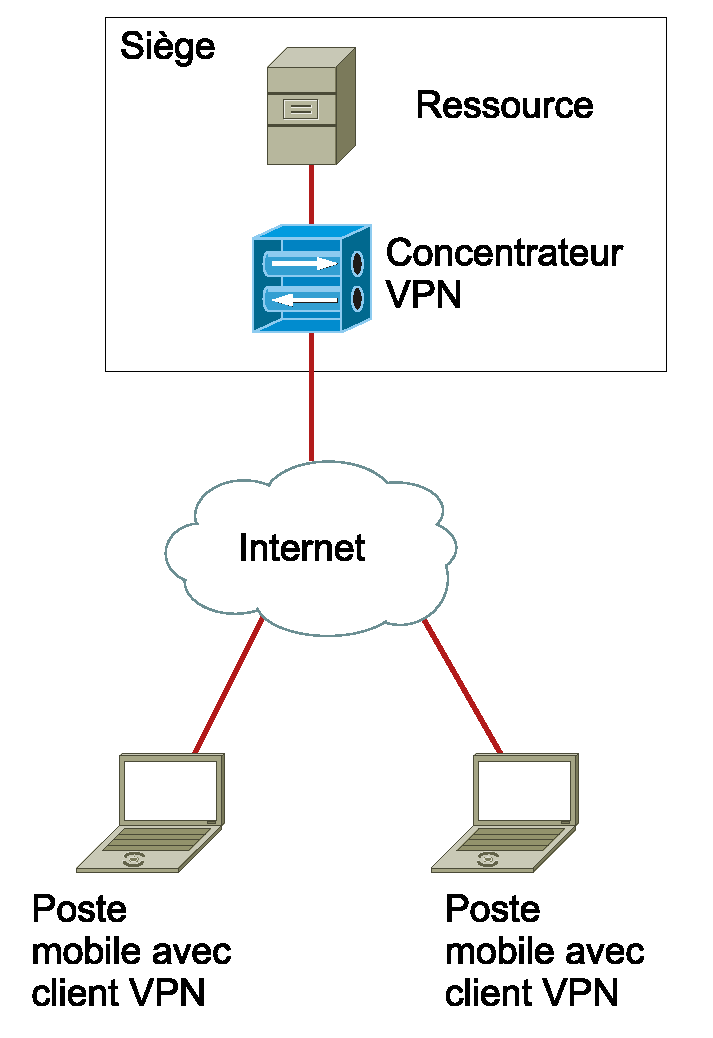
\includegraphics[width=0.4\linewidth]{OpenVPN-roadwarrior}
\end{center}
Vous remarquerez que cette utilisation ne répond pas exactement à notre besoin qui est plus complexe : Nous souhaitons interconnecter 2 réseaux IP entre eux et pas simplement donner l'accès à un poste nomade. Nous devons donc paramétrer le serveur OpenVPN pour identifier le site qui se connecte (en utilisant l'attribue «~Common Name~» du certificat SSL qui est unique pour chaque client) pour pouvoir installer les routes correspondantes aux réseaux IP de ce client :
\begin{center}
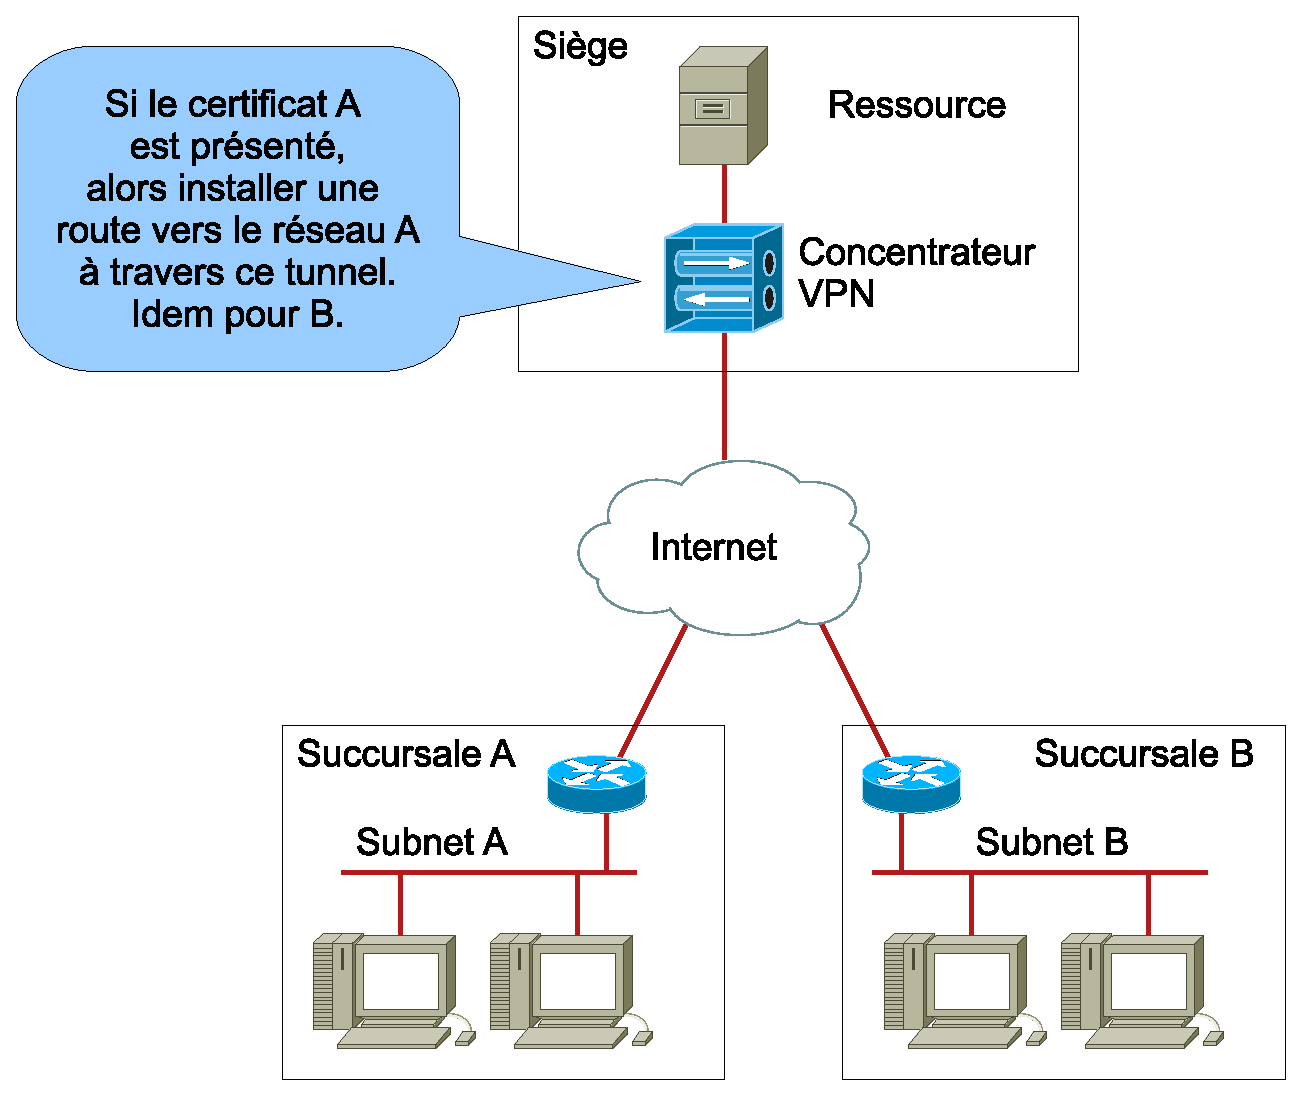
\includegraphics[width=0.7\linewidth]{OpenVPN-LAN2LAN}
\end{center}

\subsection{Génération des certificats}
Cet exercice va vous demander de créer votre propre autorité de certification et donc de générer votre fichier ca.crt : Attention de ne  pas mélanger ce nouveau avec celui de l'exercice précédent car ils portent le même nom. De plus, lors de la copie scp, vérifiez que vous n'écrasez pas un fichier déjà existant sur la machine du binôme voisin.

Générer les répertoires de clé avec la commande \shellcmd{easyrsa init-pki}. Cette commande va créer le répertoire /usr/local/share/easy-rsa/pki qui contiendra l'ensemble des certificats que vous allez créer.

Lancer le pré calcul des données pour l’algorithme de Diffie-Hellman qui servira à l’échange de clefs par la suite par la commande \shellcmd{easyrsa gen-dh}.

Puis exécutez le script \shellcmd{easyrsa build-ca nopass} et examinez le contenu du répertoire /usr/local/share/easy-rsa/pki/.

\cadre{\question{Question}
\begin{enumerate}
\setcounter{enumi}{\value{saveenum}}
\item Que s'est-il passé suite à cette commande  ?
\setcounter{saveenum}{\value{enumi}}
\end{enumerate}
}

Exécutez le script \shellcmd{easyrsa build-server-full NOM-DE-VOTRE-ROUTEUR nopass} puis examinez le contenu du répertoire pki/.

\cadre{\question{Question}
\begin{enumerate}
\setcounter{enumi}{\value{saveenum}}
\item Que s'est-il passé suite à cette commande  ?
\setcounter{saveenum}{\value{enumi}}
\end{enumerate}
}
Vous allez maintenant générer un certificat client par la commande \shellcmd{easyrsa build-client-full BINOME-? nopass} avec ? correspondant au numéro du binôme voisin.
Puis recopiez les fichiers ca.crt, dh.pem, issued/NOM-DE-VOTRE-ROUTEUR.crt et  private/NOM-DE-VOTRE-ROUTEUR.key dans le répertoire /usr/local/etc/openvpn/.
Transmettez les certificats utilisateurs (BINOME-?.crt, BINOME-?.key et ca.crt) au binôme voisin par scp.

\cadre{\question{Question}
\begin{enumerate}
\setcounter{enumi}{\value{saveenum}}
\item En quoi consistent les différentes étapes décrites dans ce chapitre ?
\item Quels sont les fichiers qui contiennent des clefs, quels types, et pour quels usages ?
\item Pourquoi n’est-ce pas utile ici de faire appel à une autorité de certification extérieure ?
\item Pourquoi une attaque de type «~man in the middle~» échouerait-elle ?
\setcounter{saveenum}{\value{enumi}}
\end{enumerate}
}

\subsection{Paramétrage d'OpenVPN}
Inspirez-vous des exemples /usr/local/share/examples/openvpn/sample-config-files/ et plus particulièrement des fichiers server.conf et client.conf pour créer votre fichier /usr/local/etc/openvpn/openvpn.conf.
La section «~Expanding the scope of the VPN to include additional machines on either the client or server subnet~» du HOW TO d'OpenVPN peux vous donner des informations supplémentaires (\textbf{www.openvpn.net/index.php/open-source/documentation/howto.html\#scope}).
Concernant le paramétrage IPv6, les variables à utiliser sont détaillées sur \textbf{www.greenie.net/ipv6/openvpn.html}.

Les paramètres obligatoires minimums au fonctionnement du daemon OpenVPN sont les suivants :
\begin{itemize}
\item Rôle et subnet à utiliser pour les tunnels eux-mêmes : server~TUNNEL-SUBNET~TUNNEL-MASK;
\item Type d'interface virtuelle à utiliser : tun;
\item Nom du fichier correspondant au certificat du CA;
\item Nom du fichier correspondant à votre certificat «~serveur~»;
\item Nom du fichier correspondant à votre clé «~serveur~»;
\item Nom du fichier qui contient les paramètres DH;
\item Route à «~pousser~» sur les clients lors de leur connexions (subnet coté serveur);
\item Nom du dossier où sont stockés les fichiers de spécification de chaque client. Dans ce dossier sera créé un fichier par client qui porte le même nom que le common-name du certificat client et ne contient qu'une déclaration : L'adresse réseau du client;
\item Routes vers les sites distants (ce sont les mêmes que dans les fichiers de l'étape précédente);
\item (optionnel) Le niveau de détail des logs : 4;
\end{itemize}

Lancer le service en ajoutant la ligne \shellcmd{openvpn\_enable="yes"} au fichier /etc/rc.conf suivis d'un \shellcmd{service openvpn start}. Utilisez les messages du fichier /var/log/messages pour résoudre vos problèmes.

\cadre{\question{Questions}
\begin{enumerate}
\setcounter{enumi}{\value{saveenum}}
\item Quelle est l'interface virtuelle créée au lancement d'OpenVPN en mode serveur ?
\item Quelles sont les routes installées suite au lancement d'OpenVPN en mode serveur ?
\setcounter{saveenum}{\value{enumi}}
\end{enumerate}
}
Demandez au binôme voisin de s'y connecter, puis une fois connecté vérifiez qu'il accède à votre serveur web.

\cadre{\question{Question}
\begin{enumerate}
\setcounter{enumi}{\value{saveenum}}
\item Comment faites-vous pour révoquer le certificat de votre utilisateur ?
\setcounter{saveenum}{\value{enumi}}
\end{enumerate}
}
%
\\
\\\emph{Appelez-les tuteurs pour qu'ils valident l'état de votre maquette.}

\end{document}
